%%%%%%%%%%%%%%%%%%%%%%%%%%%%% ANEXO %%%%%%%%%%%%%%%%%%%%%%%%%%%%%

%\section*{\centering{A – ANEXOS Y APÉNDICES }} % Añadir código
%\addcontentsline{toc}{section}{A - ANEXOS Y APÉNDICES}

% Los anexos y apéndices son materiales adicionales, utilizados para complementar el texto, añadidos al final del trabajo, con la finalidad de aclaración o de comprobación. Son elaborados por el autor y pretenden complementar una argumentación y sirven de fundamentación teórica, comprobación e ilustración (por ejemplo, mapas, leyes, códigos)

%\chapter*{Apendice A - }
%\label{ch:Apendice}

%\section*{\huge Apéndice A} 
%\section*{Fuentes de información para la descarga de MDT}
%\addcontentsline{toc}{chapter}{Apéndice A: Fuentes de información para descarga de MDT}

%\begin{itemize}
%	\item \item \url{https://www.cursosteledeteccion.com/fuentes-gratuitas-para-descargar-dem-modelo-de-elevacion-digital/}
%	\item \url{http://www.gisandbeers.com/descarga-de-dem-mundiales-mde/}
%	\item \url{https://gisgeography.com/free-global-dem-data-sources/}
%	\item \url{http://www.gpsvisualizer.com/elevation}
%	\item \url{https://mappinggis.com/2017/12/programas-gratuitos-para-trabajar-con-imagenes-de-satelite/}
%\end{itemize}

\newpage

\section*{\huge Apéndice A} 
\section*{Evolución de la Web}
\label{ch:ApendiceA}
\addcontentsline{toc}{chapter}{Apéndice A: Evolución de la Web}

\subsection{Tipos de Web} % Evolución de la Web

% hablar sobre los tipos de web, según veo hay Web 1.0, Web 2.0 y Web 3.0 o Semántica

% https://www.hazhistoria.net/blog/historia-del-www-de-la-web-10-la-web-30

% evolucion de la web: http://profesores.elo.utfsm.cl/~tarredondo/info/networks/Evolucion_Web.pdf

% Web 3.0: integración de la Web Semántica y la Web 2.0:  http://www.albertolsa.com/wp-content/uploads/2009/07/redessociales-web-30-integracion-de-la-web-semantica-y-la-web-20-los-santos-nava-godoy.pdf

\begin{figure}[H]
	\centering
	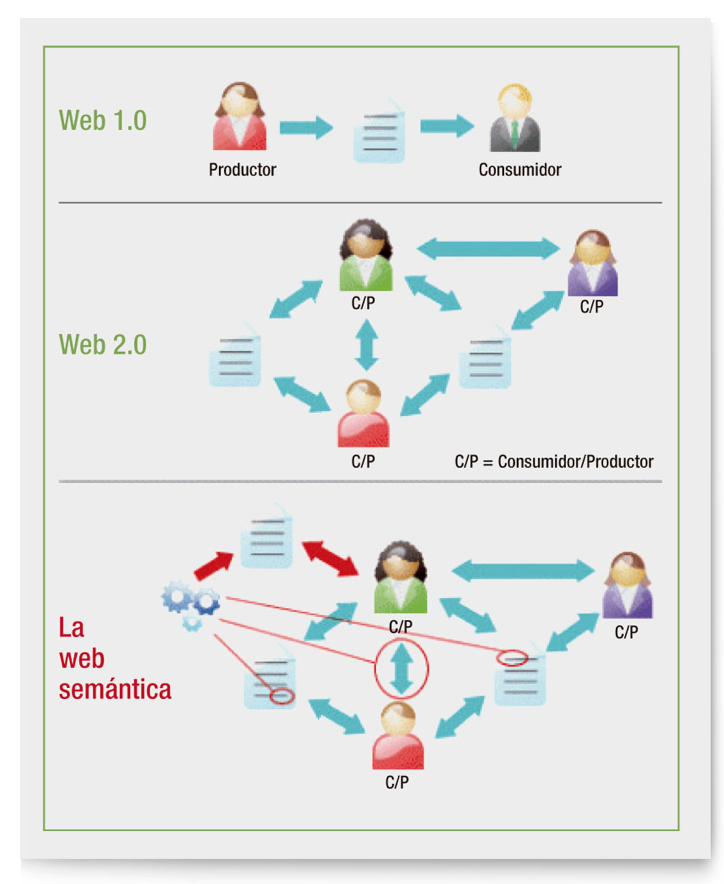
\includegraphics[height=4.5cm]{imagenes/capitulo3/10}
	\caption{}
\end{figure}
% Evolución de una web cuyo contenido es producido por unos y consumidos por otros a una web semántica que mejora la cooperación entre computadoras y humanos.

% http://www.fgcsic.es/lychnos/es_es/articulos/construyendo_una_web_semantica
A partir de ahí podemos ir saltando de una página web a otra a través de hipervínculos –estas palabras, frases, imágenes o iconos que generan la descarga automática de otra página web cuando pinchamos sobre ellos–. Esto es lo que se conoce como la web de primera generación o Web 1.0: personas con conocimiento especializado de diseño y composición de páginas web crean los documentos con su contenido y definen los hipervínculos que los entrelazan; los usuarios no expertos son fundamentalmente consumidores de información. Leen noticias, consultan diccionarios, visualizan imágenes o vídeos o compran productos. 

% http://www.fgcsic.es/lychnos/es_es/articulos/construyendo_una_web_semantica
En la web de segunda generación, la Web 2.0, los usuarios no expertos, además de consumidores, pueden ser también generadores de contenidos y proveedores de servicios. Mediante blogs, por ejemplo, se pueden escribir y compartir reflexiones periódicas, y los lectores pueden añadir comentarios o nuevos enlaces relevantes; con Wikipedia, millones de personas construyen una gran enciclopedia multilingüe que constantemente es actualizada y ampliada por los propios usuarios; a través de redes entre pares, como originalmente Napster, BitTorrent o eMule, se comparten películas y ficheros de música; y últimamente, con la irrupción de las redes sociales —Facebook, Tuenti o Twitter—, la Web se ha convertido en un espacio global de participación e interacción entre usuarios.

% https://disenowebakus.net/semantica-web.php
Las funcionalidades de creación de contenidos textuales y audiovisuales y la comunicación entre individuos y grupos cristalizó en una nueva generación de herramientas conocida como Web 2.0 o Web social, orientadas a facilitar la conexión entre las personas. El factor humano dejó de ser un elemento pasivo para convertirse en una agente activo en la Web. La idea fundamental se centra en el establecimiento de redes o comunidades de usuarios que trabajan con una serie de servicios basados en aplicaciones Web como los blogs, los servicios de publicación de contenidos multimedia, las redes sociales o las wikis. Se trata de un uso concreto de la Web, que fomenta la colaboración para difundir e intercambiar información de forma rápida y sencilla. Sin embargo, hemos de tener en cuenta que esta situación implica una serie de problemas derivados de la propia naturaleza de una Web en la que participan los usuarios. Existen cantidades enormes de recursos desorganizados, duplicados o desactualizados, entre los que encontrar la información buscada termina resultando un trabajo arduo. Los motores de búsqueda Web, aunque han mejorado en los últimos años, continúan catalogando sólo una porción pequeña de la Web y a veces producen resultados que no son pertinentes y a menudo inexactos o imposibles de encontrar. Esto se debe a que la cantidad, estructura y originalidad de contenidos en la Web no han evolucionado paralelamente a como lo han hecho los procesos de publicación de los mismos. Existen gran cantidad de páginas duplicadas, puesto que muchos usuarios prefieren copiar contenidos en vez de referenciarlos con enlaces de hipertexto. Multitud de páginas hacen un uso incorrecto de metadados HTML, distorsionando su utilidad en los procesos de búsqueda. Tampoco es posible distinguir en todos los casos el tipo de recurso recuperado durante la búsqueda: un documento informativo, una ficha de una aplicación en un servicio de descarga de pago, una entrada en un foro de debate, etc. En este contexto, los buscadores Web son incapaces en ocasiones de ofrecer unos resultados útiles. 


% http://www.fgcsic.es/lychnos/es_es/articulos/construyendo_una_web_semantica
La web semántica viene a ser la tercera generación de la Web, la Web 3.0, una extensión de la Web actual en la que los contenidos están organizados de forma que no solo los humanos sino también las computadoras sean capaces de procesar su significado —por eso lo de semántica— posibilitando así una mejor cooperación entre computadoras y humanos. La nomenclatura Web 1.0, 2.0 y 3.0 es seguramente artificiosa, ya que de hecho no se trata de nuevas versiones de la Web, sino de la misma web de siempre pero con niveles añadidos de funcionalidad. 

% https://www.weblaspalmas.es/noticias-tecnologicas/172/La-web-3-0-De-la-web-social-a-la-semantica.html

% Meter algo en el principio de este apartado y luego continuar escribiendo en el apartado de la web semántica
% http://personales.upv.es/ccarrasc/doc/2002-2003/WebSem/WS_2_b.htm#_Toc41588970

% Las web 3.0: de la web social a la semántica: https://www.puromarketing.com/12/15656/social-semantica.html

% https://disenowebakus.net/semantica-web.php
Desde el punto de vista de la recuperación de información en la Web se precisa el uso de metadatos, que apliquen modelos estándar para la descripción de los recursos. Además, su desarrollo y uso mejoraría no solamente los buscadores Web, sino también ampliarían los horizontes de la Web para el intercambio y procesamiento de datos entre aplicaciones de forma automática. Hace algún tiempo que el XML ha venido utilizándose para el intercambio de datos a fin de que estos sean interoperables a nivel sintáctico. Sin embargo, la Web semántica plantea el uso de un modelo de datos básicos como es el RDF que amplía la interoperabilidad a nivel semántico. Además la Web semántica se organiza en una estructura multinivel que va desde la simple descripción de recursos mediante metadatos a la definición de ontologías y reglas de inferencia.


% https://disenowebakus.net/semantica-web.php
Ya no estamos hablando de un sistema para publicar y comunicar resultados de experimentos y trabajos de investigación. Sobre aquella Web, se basada en la interconexión de documentos mediante enlaces de hipertexto, se han creado nuevas herramientas gracias al desarrollo de lenguajes de programación para la Web y su integración con sistemas de base de datos. El concepto de Sistema de Gestión de Contenidos plantea la Web como una plataforma universal para la creación de todo tipo de herramientas, cuyo uso únicamente precisa del usuario un sólo software esencial: el navegador Web. Los usuarios comenzaron a interactuar con la Web más allá de la búsqueda y consulta de información.




